\documentclass{article}

\usepackage{fancyhdr}
\usepackage{ragged2e}
\usepackage{graphicx}
\usepackage{caption}
\usepackage{geometry}
\usepackage{amsmath}
\usepackage{rotating}

\usepackage{listings}
\usepackage{color}

\definecolor{dkgreen}{rgb}{0,0.6,0}
\definecolor{gray}{rgb}{0.5,0.5,0.5}
\definecolor{mauve}{rgb}{0.58,0,0.82}

\lstset{frame=tb,
  language=Java,
  aboveskip=3mm,
  belowskip=3mm,
  showstringspaces=false,
  columns=flexible,
  basicstyle={\small\ttfamily},
  numbers=none,
  numberstyle=\tiny\color{gray},
  keywordstyle=\color{blue},
  commentstyle=\color{dkgreen},
  stringstyle=\color{mauve},
  breaklines=true,
  breakatwhitespace=true,
  tabsize=4
}

\setcounter{secnumdepth}{1}

\usepackage{chngcntr}
\counterwithin{figure}{section}

\renewcommand*{\thepage}{C\arabic{page}}

\pagestyle{fancy}
\lhead{ACME Robotics}
\chead{\#8367}
\rhead{\ifcontents Contents \else Week \thesection \fi}

\newif\ifcontents
\contentstrue

\makeatletter
\renewcommand{\@seccntformat}[1]{}
\makeatother

\begin{document}\contentsfalse

\subsection{Work with intake prototypes.}
%! Test intake prototypes. 
After looking further into the dual flywheel intake design, Jon and Kelly decided this was not a practical option because it would be difficult to fit onto the robot and create an efficient chain setup. Kelly and Jon then decided to go with a swing down roller design, as this would be easy to fit into the existing design and will likely work just as well. After deciding this, Jon built a prototype for this new intake. 

\begin{figure}
    \centering
    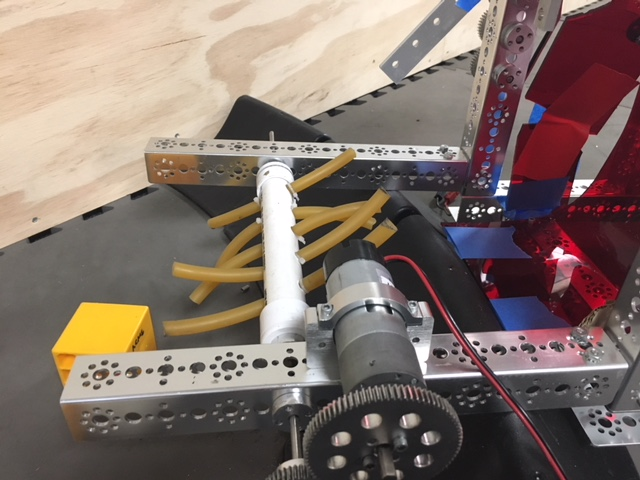
\includegraphics[width=.6\textwidth]{03_09-17/images/IMG_0262.JPG}
    \caption{Deploy-able intake prototype}
    \label{fig:my_label}
\end{figure}

\subsection{Develop a Team Marker}
%! Design a team marker that will be used at the tournaments.
Shawn and Ben were tasked with developing a team marker. The team marker should fit within the size constraints and, ideally represent something about the team. Ben and Shawn decided to make a prototype anvil marker that could roll. Ben sketched out an anvil in his notebook and measured the height of cardboard. Based on this measurement, he divided the drawing into equal sections that were that height. Shawn the cut out the cardboard pieces and they pieced it together.
\end{document}